\subsection{Results for Co-discovery}
The functionality primarily used while trying to solve the assignments was the main search bar, located at the top center, see the red square in \autoref{results:amazonsearchbar}, and the sorting function of the found results for a given search, sorted primarily by price, see the red square in \autoref{results:amazonsortby}.

\begin{figure}[h]

\includegraphics[scale=0.3]{./includes/amazon_search_bar.png}
\caption{Amazon main search bar}
\label{results:amazonsearchbar}
\end{figure}

\begin{figure}[h]
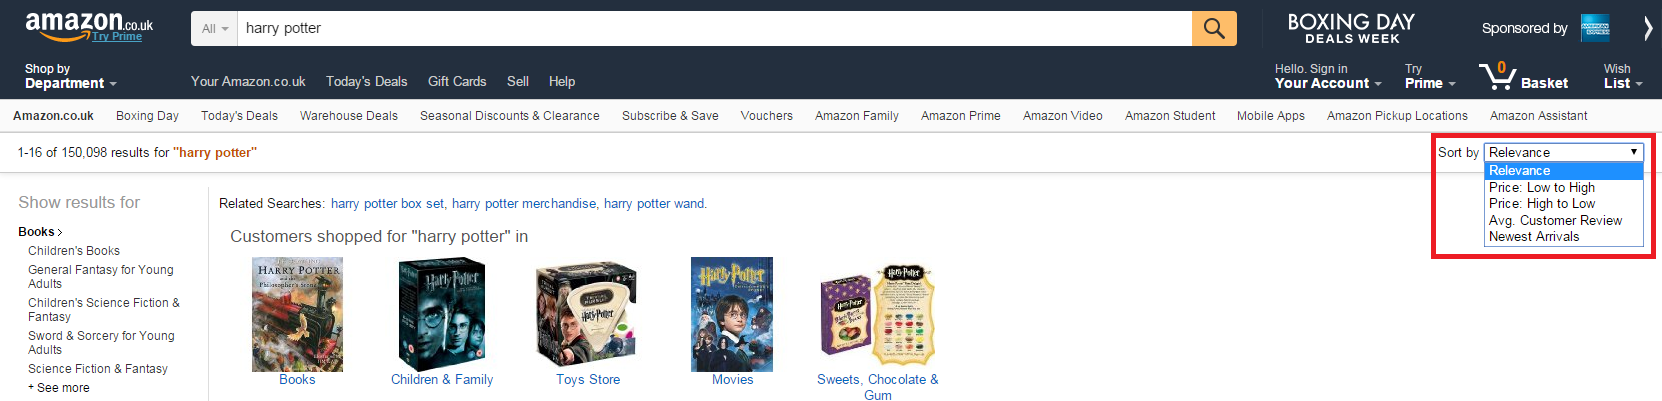
\includegraphics[scale=0.3]{./includes/amazon_sort_by.png}
\caption{Amazon sort search result by}
\label{results:amazonsortby}
\end{figure}

The functionality that we considered useful, and expected to be used, included the recommender system, and the category drop-down menu in the top left corner, which were never utilized, see the blue square in \autoref{results:amazonsearchbar} and the red square in \autoref{results:amazonrecommender}. Also the participants became rather confused when trying to find the relevant information regarding shipping of a certain product.

\begin{figure}[H]
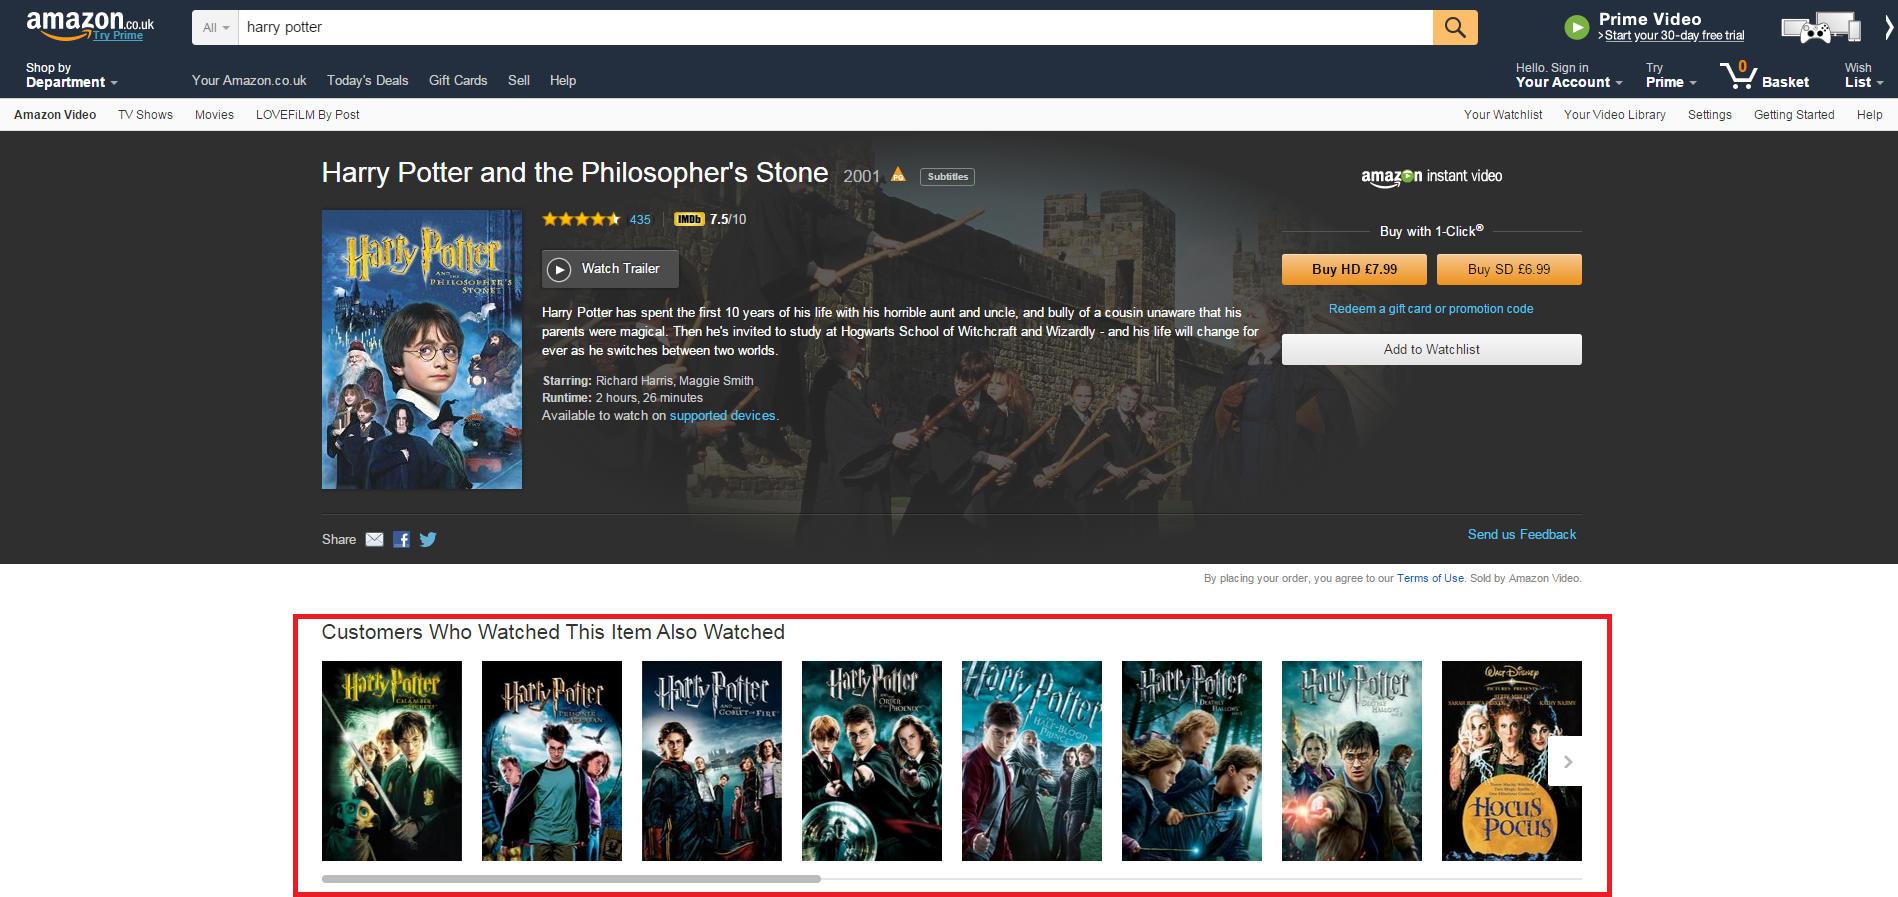
\includegraphics[scale=0.265]{./includes/amazon_recommender}
\caption{Amazon recommender system}
\label{results:amazonrecommender}
\end{figure}


\subsection{Results for AttrakDiff}
From the results of the AttrakDiff questionare we observed that the participants agreed that the system was
\begin{itemize}
\item Simple
\item Easy to use
\item Practical
\item Professional
\end{itemize}
We suspect this is because the assignments were solved using primarily the search bar, which means that the more complex functionality of Amazon was never used. However they didn't find the system particularly:
\begin{itemize}
\item Social
\item Innovative
\item Creative
\item New
\end{itemize}
This is likely because the purpose of the system is by large pragmatic.